\documentclass[11pt, oneside]{article} 
\usepackage{geometry}
\geometry{letterpaper} 
\usepackage{graphicx}
	
\usepackage{amssymb}
\usepackage{amsmath}
\usepackage{parskip}
\usepackage{color}
\usepackage{hyperref}

\graphicspath{{/Users/telliott_admin/Dropbox/Tex/png/}}
% \begin{center} 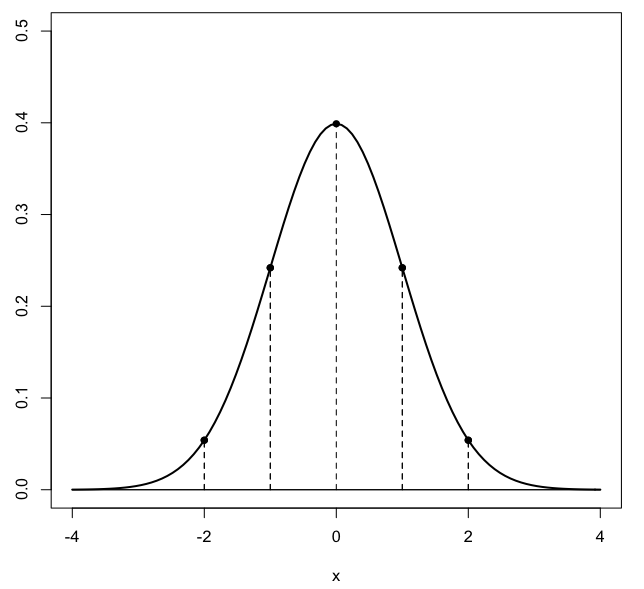
\includegraphics [scale=0.4] {gauss3.png} \end{center}

%break
\title{Polar parabola}
\date{}

\begin{document}
\maketitle
\Large
\label{sec:Polar_parabola}
\subsection*{foucs and directrix}
A classical approach to conic sections is that of the focus and the directrix.  The directrix is defined as a straight line, for convenience we will make it a horizontal line passing below the $x$-axis, and the focus as a point on the axis of symmetry above the vertex.
\begin{center} 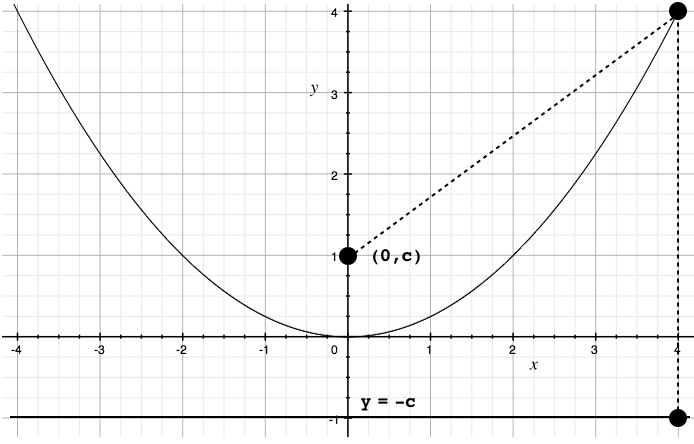
\includegraphics [scale=0.4] {para3.png} \end{center}
These are positioned so that the distance $c$ from the vertex to the focus is the same as the distance from the vertex vertically down to the directrix.  (This $c$ is \emph{not} the same as the one in the standard formula for a parabola:  $ax^2 + bx + c$).

The claim is that for the correct value of $c$, the distance from any point on the parabola to the focus will be equal to the distance vertically down to the directrix.

The parabola shown has the equation $y=\frac{1}{4}x^2$.  That is, $a = \frac{1}{4}$.  For this parabola, $c=1$.

To derive this result, consider a general point on the parabola, $Q=(x,y)$.  The vertical distance down to the directrix is 
\[ y + c \]
The distance to the focus is given by Pythagoras
\[  d = \sqrt{x^2 + (y - c)^2} \]

The constraint is that these two distances should be equal, so the squares should also be equal
\[ (y + c)^2 = x^2 + (y - c)^2 \]
At this point we recall this result from algebra 
\[ (a+b)^2 - (a - b)^2 = 4ab \]
Thus
\[ (y + c)^2 = x^2 + (y - c)^2 \]
becomes
\[ 4ayc = x^2 \]
\[  4ac = 1 \]
For example, if $a = 1$, $c = \frac{1}{4}$ as we had above.

\subsection*{polar coordinates}
To derive an equation for the parabola in polar coordinates, it is convenient to rotate it by a quarter-turn (now $x = y^2$), and to move it so that the focus is at the origin.

\begin{center} 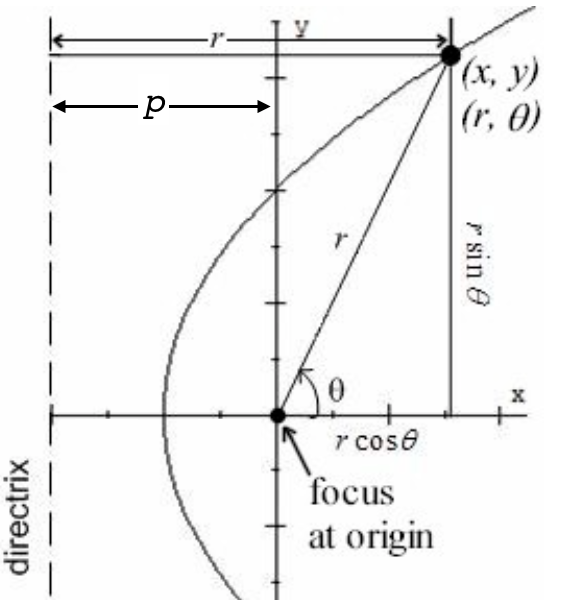
\includegraphics [scale=0.35] {parabola_parametric.png} \end{center}
$r$ is simply the distance from the origin to the point $x,y$.  We use the constraint that this distance is equal to the distance from the point to the line of the directrix.

Standard notation is that the distance from the focus to the directrix is $p$.  Half that distance is $c$, so the whole distance is $p = 2c$.  Since
\[ p + r \cos \theta \]
is the horizontal distance from the point to the directrix, we have that
\[ r = p + r \cos \theta \]
\[ r = \frac{p}{1- \cos \theta} \]

Since $p = 2c$ and $4ca = 1$, as an example, if we have $a=1$, then $p$ = $1/2$ so
\[ r = \frac{1/2}{1- \cos \theta} \]
\[ r = \frac{1}{2- 2 \cos \theta} \]

To go back to the Cartesian ($xy$) form, write
\[ \frac{x}{r} = \cos \theta \]
We had
\[ r = \frac{p}{1- \cos \theta} \]
So
\[ r = \frac{p}{1- x/r} \]
\[ r - x = p \]
\[ r = x + p \]
\[ r^2 = x^2 + y^2 = (x + p)^2 \]
\[ x^2 + y^2 = x^2 + 2xp + p^2 \]
\[ y^2 = 2p(x + p/2) \]
so
\[ \frac{1}{2p} y^2 = x + p/2 \]

Recall that this parabola had its origin shifted to the right:  $h = p/2 = c$, and the $x$-coordinate of the vertex is $-c$, so we have to add $c$ back to $x$.

Now, set $4ca = 2pa = 1$ to recover $(x+c) = ay^2$.

\end{document}